%
% pathfinding user interfaces
% @author Tobias Weber <tweber@ill.fr>
% @date july-2021
% @license see 'LICENSE' file
%

\chapter{Graphical and Scripting User Interfaces}
\label{ch:gui}
The present chapter describes the different user and developer interfaces to the software of the present work.

The software has been realised in a modular fashion, it comprises a core
module, which was introduced in chapter \ref{ch:impl} and which can be easily used as a library 
and linked into external C++ applications. 
More details on directly employing the core library can be found in section \ref{sec:library}.
Such a library usage will be important in the future when we plan to utilise the software as a 
plug-in module to the instrument control software \textit{NOMAD} \cite{web_NOMAD} that is 
employed at the Institut Laue-Langevin.

Furthermore, a graphical user interface (GUI) has been implemented for a visual and interactive 
representation of the instrument and the underlying algorithms and to facilitate their use. 
The GUI is described in detail in section \ref{sec:gui}.

Finally, the software allows scripting via \textit{Python} \cite{Rossum2011, web_python}. 
Apart from simply setting up a workflow and plotting the results, the \textit{Python} interface 
aims to allow the usage of the software in \textit{Python}-based instrument control systems such as 
\textit{NICOS} \cite{web_NICOS}, which is used at the Forschungsreaktor M\"unchen II (FRM-II). 
Details on the scripting interface can be found in section \ref{sec:scripting}.



\section{Core module and C++ library}
\label{sec:library}
The core module contains all necessary calculation as well as input and output sub-modules. 
Here, we only describe the latter two, since the computation functionality of the core module 
has already been treated in detail in chapter \ref{ch:impl}.

The instrument configuration is read from an \textit{XML} file whose hierarchical structure
mirrors the internal data organisation of the core module and its class hierarchy.
The \textit{XML} file is parsed using the \textit{Boost.PropertyTree} library \cite{web_boost_proptree}
and objects are created of the respective classes once the corresponding section in the \textit{XML}
structure is discovered. An \textit{XML} section is handed down to the corresponding C++ object,
so that each object only receives the portions of the \textit{XML} configuration it is responsible for.
Editing the \textit{XML} instrument configurations can be done using the GUI module of section \ref{sec:gui}.

While the central \lstinline[language=C++]|PathBuilder| class offers getter functions for all intermediate
data that is generated during each step of the calculation workflow, the final results are output using
the classes derived from the purely virtual class \lstinline[language=C++]|PathsExporterBase| that resides
in the files \lstinline|./src/core/PathsExporter[.h,.cpp]|. Currently, three possible output classes
are available:
\begin{itemize}
	\item \lstinline[language=C++]|PathsExporterRaw|, which outputs the vertices of the calculated 
		final instrument path in a raw text format.
	\item \lstinline[language=C++]|PathsExporterNomad|, which writes out commands for driving the
		motors of instruments which are controlled by the \textit{NOMAD} software \cite{web_NOMAD}.
	\item \lstinline[language=C++]|PathsExporterNicos|, which generates \textit{Python} code to
		be used for driving the instrument using the \textit{NICOS} \cite{web_NICOS} control system.
\end{itemize}
For easy extensibility and to isolate the \lstinline[language=C++]|PathBuilder| class from the output
code, the output class hierarchy is realised using the Visitor pattern \cite{wiki_visitor} 
\cite[Ch. 4, pp. 141-147]{FUH_prog2019}, where the \lstinline[language=C++]|PathBuilder| 
accepts the output base class and dispatches to the desired child object.

The core module functionality is self-contained and does, for instance, not depend on any GUI code.
It is therefore straightforward to statically or dynamically link it to external applications which 
wish to use the pathfinding functionality. To avoid exposing the user to the complexities of
the C++ language, a more comfortable approach is provided by both the graphical as well 
as the \textit{Python} interface, which are described in the following sections.



\section{Graphical user interface}
\label{sec:gui}
The software's main graphical user interface (GUI) is based on the \textit{Qt} framework 
\cite{web_Qt}, that allows for an easy and rapid cross-platform GUI development in C++. 
Both current releases of \textit{Qt} are supported, namely version 5 and version 6.
Fig. \ref{fig:gui} depicts a typical session of the GUI.
Similar to the core calculation module, the GUI is written in the recent C++20
standard \cite{ISOCPP20} of the C++ language family \cite{Stroustrup2008, Stroustrup2018}.
The source code of the GUI module can be found in the directory \lstinline|./src/gui| of the
source repository, see chapter \ref{ch:online} for more information.

\begin{figure}[htb]
		\begin{center}
			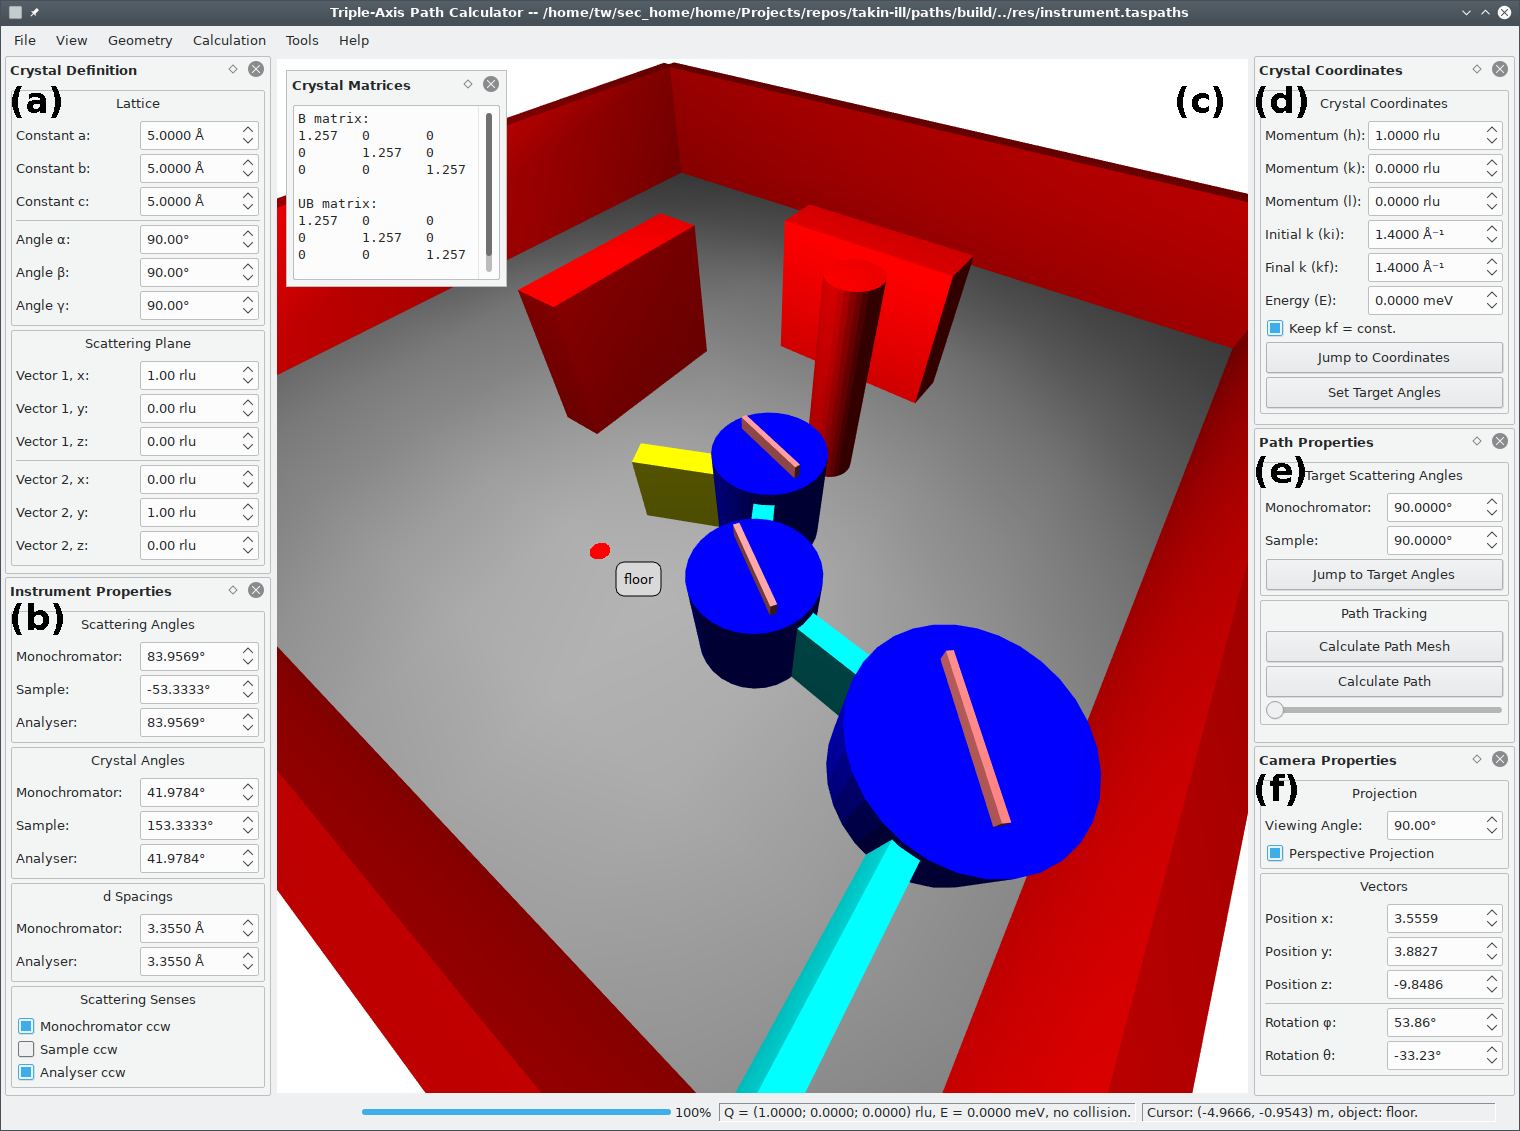
\includegraphics[width = 1 \textwidth]{figures/gui}
		\end{center}
	\caption[Main program GUI.]{Main GUI. 
		Here, instrument and sample crystal properties can be set up,
		walls can be added and moved. 
		Furthermore, paths around the walls can be calculated.
		The central view provides a three-dimensional visualisation of the instrument
		configuration and is fully dynamic: Each element, including the instrument
		and the wall segments, can be moved or manipulated using the mouse.
		See the text for a description of each interface element.
		\label{fig:gui}}
\end{figure}

The functions of the individual control elements of the main GUI, which are marked as (a)-(f)
in Fig. \ref{fig:gui}, are explained in the following sections. Each of the panels corresponds to a specific
functionality of the core module (chapter \ref{ch:impl}), to which all calculations are delegated. 
This way, the GUI is literally just an interface and only performs auxiliary calculations.
By the same token, the core module itself is completely independent of the GUI, or any other
interface code, and the full functionality of the software, except GUI-specific visualisation and editing
capabilities, is equally accessible from the other alternative interface modules, e.g. the \textit{Python}
interface described in section \ref{sec:scripting}, or the raw C++ library interface.



\subsection{Crystal definition dock window}
\label{sec:gui_xtal}
\begin{minipage}{1 \textwidth}
\setlength{\intextsep}{0.25cm}
\begin{wrapfigure}{r}{0.46 \textwidth}
	\vspace{-0.25cm}
	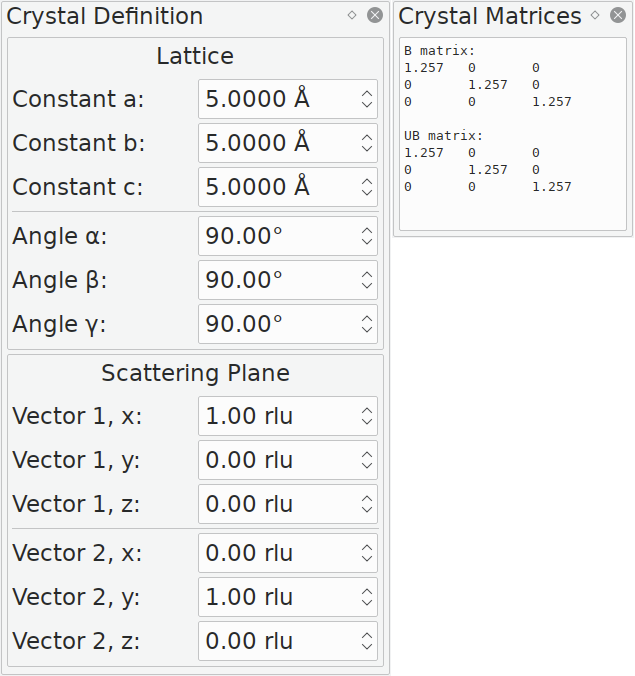
\includegraphics[width = 0.45 \textwidth]{figures/gui_xtal}
	\caption[Crystal definition window.]{Crystal definition window (a).
		\label{fig:gui_xtal}}
\end{wrapfigure}

Dock window (a) of the main GUI (Fig. \ref{fig:gui}) sets up the metric tensor corresponding 
to the crystal $UB$ matrix using the sample definition.
A magnified view of this window is provided in Fig. \ref{fig:gui_xtal}. 
As seen before, the $UB$ matrix transforms the crystal coordinate system into the instrument's 
laboratory coordinate system.
The necessary information for the $B$ matrix comprise the axis lengths of the sample lattice's
unit cell as well as the axis angles for the non-Cartesian crystal coordinate system.
The $UB$ matrix rotates the crystal coordinate system so that the $x$ and $y$ axes correspond
to the 2-d scattering plane accessible by the instrument.
The mathematical background to this formalism has been discussed in chapter \ref{ch:xtal}.
Finally, the $B$ and $UB$ matrices calculated from the entered crystal information are shown 
in the floating window right of (a).
\end{minipage}
\vspace{0.5cm}



\subsection{Instrument properties dock window}
\begin{minipage}{1 \textwidth}
\setlength{\intextsep}{0.25cm}
\begin{wrapfigure}{l}{0.3 \textwidth}
	\vspace{-0.25cm}
	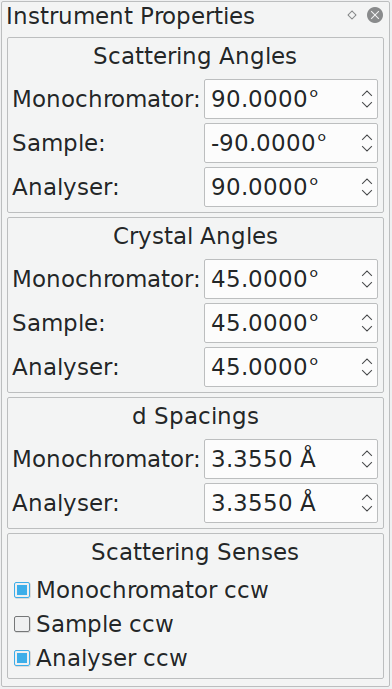
\includegraphics[width = 0.25 \textwidth]{figures/gui_instrument}
	\caption[Instrument properties window.]{Instrument properties window (b).
		\label{fig:gui_instr}}
\end{wrapfigure}

The raw instrument properties, which are agnostic of any sample crystal coordinates, are set up
using the dock window shown in Fig. \ref{fig:gui_instr}. It displays and lets the user modify
any crystal rotation angles, both the rocking angles of the crystals around their own axes
as well as the scattering angle with respect to the following axis. These angles and their
use in diffraction (two-axis) and spectroscopy (three-axis) instruments has been described 
in chapters \ref{ch:intro} and \ref{ch:xtal}. 
The fields names ``$d$ spacings'' correspond to the spacing of the crystal planes in the 
monochromator and analyser crystals. In our examples we use the value of $d\,=\,3.355\, \textup{\AA}$
which corresponds to scattering on the $\left(002\right)$ Bragg reflection of highly oriented
pyrolithic graphite (HOPG) \cite[p. 250]{Shirane2002}, which is one of the standard crystals used as a
monochromator or analyser in a TAS instrument.
Finally, the check boxes named ``scattering senses'' control the sign of the scattering angles.
If the box is checked, a positive angle corresponds to a counterclockwise sense, i.e. corresponding
to the usual mathematical definition, and alternatively to a clockwise sense when unchecked.
From the standpoint of the physics to be studied in the sample, these signs have no influence
in practice. They do, however, strongly affect the resolution of the instrument \cite{Eckold2014}
and have to be considered carefully in the set-up of an experiment.
\end{minipage}



\subsection{Main workspace}
\label{sec:gui_gl}
The largest portion of the screen is reserved for the main workspace.
A typical view is shown in element (c) of Fig. \ref{fig:gui}.
Here, a graphical representation of the instrument space containing the instrument and the walls 
is performed using \textit{OpenGL} \cite{web_OpenGL} via \textit{Qt}'s
\lstinline[language=C++]|QOpenGLWidget| \cite{web_QOpenGLWidget} class.
The current view of the instrument is controlled by moving the mouse while holding the right button.
The camera position, viewing angle and direction as well as the type of projection matrix are 
displayed in dock window (f) and can also be entered directly.

The workspace is not restricted to a passive view of the instrument, but also functions as an editor
which allows an easy interaction with the 3-d objects in the scene. For example, wall segments can
be inserted, edited and removed on the fly, see Fig. \ref{fig:gui_objects}.
The segments as well as the instrument axes themselves can be dynamically moved by dragging them using the 
mouse. This is realised by ``unprojecting'' the current mouse position from its coordinates with respect 
to the near and far planes of view frustum into the global object coordinate system in a first step, 
and finding all objects that intersect with a line through these two unprojected points in a second step. 
Mathematical details on this and other aspects of \textit{OpenGL} rendering have been discussed 
in chapter \ref{ch:gl}.
The renderer itself can be found in the class \lstinline[language=C++]|PathsRenderer|, located in
the file \lstinline|./src/gui/PathsRenderer.cpp|.

Internally, several data structures are maintained for the object system. 
The main hierarchical object system has its root in the \lstinline[language=C++]|InstrumentSpace|
class. This class is part of the core module (see chapter \ref{sec:tasmodel}) and is not dependent
on \textit{OpenGL} or the GUI.
To avoid introducing GUI- or rendering-specific details into the core, a second object
system is maintained in the GUI's \lstinline[language=C++]|PathsRenderer| itself. 
Here, all the \textit{OpenGL}-specific details, for example the vertex array objects \cite{wiki_vao} 
of all 3-d objects that are displayed on the screen, are stored.
Data in this secondary object system is updated automatically as soon as the user edits an object 
property from the main \lstinline[language=C++]|InstrumentSpace| instance.


\begin{figure}[htb]
	\begin{minipage}{0.45 \textwidth}
		\begin{center}
			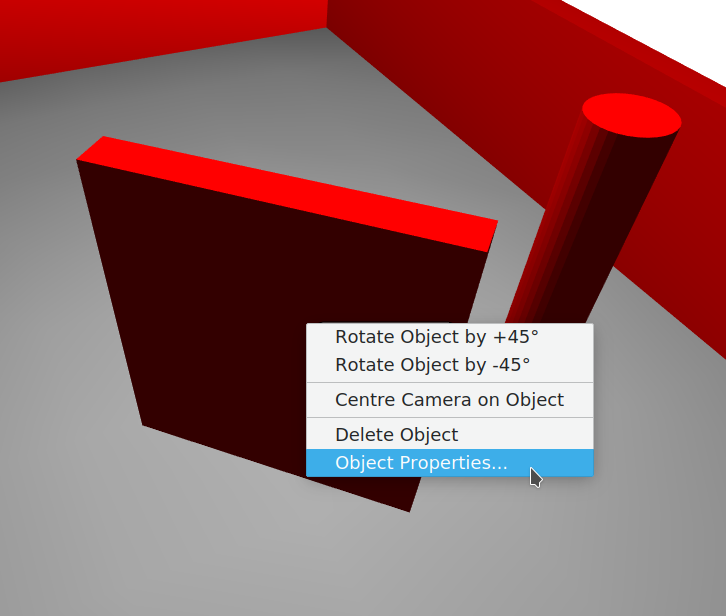
\includegraphics[width = 1 \textwidth]{figures/gui_object}
		\end{center}
	\end{minipage}
	\hspace{0.1cm}
	\begin{minipage}{0.5 \textwidth}
		\begin{center}
			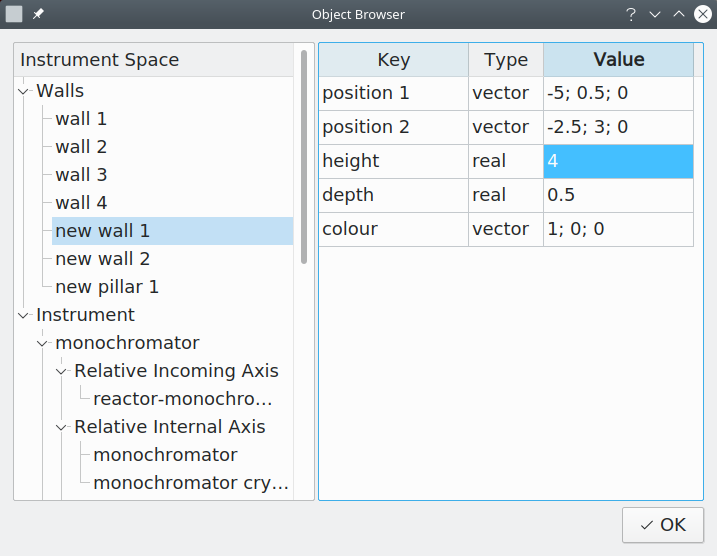
\includegraphics[width = 1 \textwidth]{figures/gui_objbrowser}
		\end{center}
	\end{minipage}
	\caption[Object manipulation.]{Manipulation of 3-d objects in the main GUI.
		Left panel: Objects can be moved by mouse and possess a context menu.
		Right panel: All objects in the instrument space are organised hierarchically. 
			Their properties can be dynamically edited.
		\label{fig:gui_objects}}
\end{figure}



\subsection{Crystal coordinates dock window}
\label{sec:gui_xtalcoords}
\begin{minipage}{1 \textwidth}
\setlength{\intextsep}{0.25cm}
\begin{wrapfigure}{r}{0.26 \textwidth}
	\vspace{-0.25cm}
	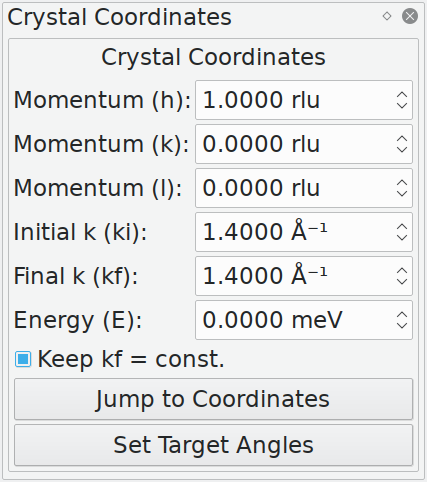
\includegraphics[width = 0.25 \textwidth]{figures/gui_xtalcoords}
	\caption[Crystal coordinates window.]{Crystal coordinates window (d).
		\label{fig:gui_xtalcoords}}
\end{wrapfigure}

Using the $UB$ transformation matrix that has been set up before (chapter \ref{sec:gui_xtal}),
an instrument position can be entered in the crystal coordinates dock window, which is
shown in Fig. \ref{fig:gui_xtalcoords}.
At triple-axis spectrometers, coordinates are given as four-dimensional tuples of the
form $\left(h\  k\  l\  E \right)^t$, where the three-dimensional momentum transfer
vector in the coordinate system of the instrument and its relation to the initial and final
wavevectors $\underline{k}_i$ and $\underline{k}_f$, is thus \cite[p. 11]{Shirane2002} \cite{Lumsden2005}
\begin{equation}
	\underline{Q}\ =\ UB\cdot \left(\begin{array}{c} h \\ k \\ l \end{array}\right) \ \equiv\ \underline{k}_i - \underline{k}_f.
\end{equation}
The fourth coordinate component, namely the energy transferred to the crystal, is \cite[p. 11]{Shirane2002}
\begin{equation}
	E \ =\ \frac{\left( \hbar k_i \right)^2}{2 m_n} - \frac{\left( \hbar k_f \right)^2}{2 m_n}.
\end{equation}
The checkbox labelled ``keep $k_f$ = const'' selects which one of the two wavenumbers, the incoming ($k_i$) 
or the outgoing ($k_f$), is kept constant and which is variable to effectuate the energy transfer
from the neutron to the sample.
Depending on the selected mode, the configuration space and motion planning calculations will either involve
the monochromator scattering angle (in case $k_f$ chosen to be constant), or the analyser scattering
angle (in case $k_i$ is chosen to be constant).
Please refer to chapters \ref{ch:intro} and \ref{ch:xtal} for details on the calculations and physical background.

The button labelled ``jump to coordinates'' sets the current (and initial path position)
of the instrument to the given crystal coordinates, whereas the ``set target angles'' button
sets the target position on the instrument path.

\end{minipage}



\subsection{Path properties dock window and dialog}
\begin{minipage}{1 \textwidth}
\setlength{\intextsep}{0.25cm}
\begin{wrapfigure}{l}{0.26 \textwidth}
	\vspace{-0.25cm}
	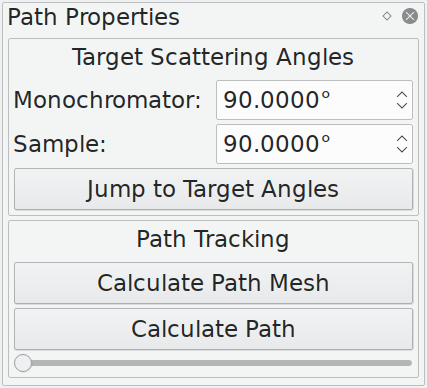
\includegraphics[width = 0.25 \textwidth]{figures/gui_path}
	\caption[Path properties window.]{Path properties window (e).
		\label{fig:gui_path}}
\end{wrapfigure}

Finally, the calculation of the instrument path is done using the path properties dock window
given in Fig. \ref{fig:gui_path}. Here, the target scattering angles are calculated from the crystal
coordinates and set by the previous step (section \ref{sec:gui_xtalcoords}). For direct positioning,
the angles can also be entered manually, thereby overriding the crystal coordinate calculations.

The button labelled ``calculate path mesh'' starts the calculation of the skeletal bisectors that are
described in chapter \ref{sec:polygonal_voronoi_diagram}.
Once a path mesh is available, the ``calculate path'' button finds the optimal path on the mesh and 
invokes the core library functions described in chapter \ref{sec:exepath}.
As soon as a path has been calculated, its positions can be tracked using the progress bar at the bottom
of the dock window.

Details on the path calculations, including the path mesh, are displayed in the angular configuration
space dialog that is depicted in Fig. \ref{fig:gui_configspace}.
Here, the start and target positions can also be directly dragged and dropped via mouse and the
effects on the calculation are visualised live.
The library \textit{QCustomPlot} \cite{web_QCustomPlot} is used for plotting.

\end{minipage}



\begin{figure}[htb]
		\begin{center}
			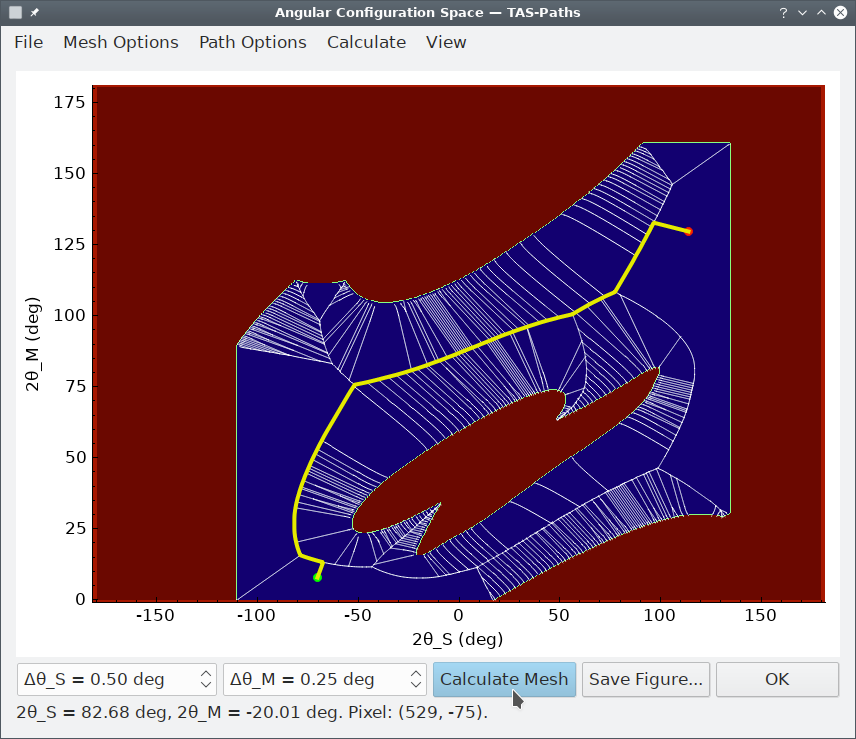
\includegraphics[width = 0.75 \textwidth]{figures/gui_configspace}
		\end{center}
	\caption[Configuration space dialog.]{Angular configuration space and path calculation dialog.
	Using the \textit{QCustomPlot} library \cite{web_QCustomPlot}, the dialog plots all possible
	instrument positions for the monochromator and sample scattering angles, $2\theta_M$ and $2\theta_S$, respectively.
	Forbidden positions are shown in red.
	These can be invalid angles as well as collisions of the instrument with walls
	(here, specifically, the pillar from Fig \ref{fig:gui}), or with itself.
	Allowed positions are drawn in blue. The mesh of all possible instrument
	paths is shown as white lines, while a currently selected example path from
	the red start to the green target position is shown as a yellow line.
		\label{fig:gui_configspace}}
\end{figure}


\subsection{Case study and illustrative example}
We proceed to present an illustrative example modelled after a situation that arose during an 
experiment that we performed at the instrument \textit{Thales} \cite{thales} some time ago. 
The situation is an archetypical one which often arises during a measurement and which
can be automatised and visualised using the present software.
The software was not yet available at the time of the experiment, though, so we still had to resort 
to long-winded manual driving of the instrument.

\paragraph{Problem}
After a series of scans, the instrument reached a position of 
$Q_\mathrm{start}\,=\,\left(1.5,\ 1.5,\ 0.5\right)\, \mathrm{rlu}$ and  $E_\mathrm{start}\,=\,10\, \mathrm{meV}$, where
$Q$ and $E$ refer to the momentum and energy transfer from the neutron to the crystal, respectively,
and ``rlu'' stands for \textit{relative lattice units}, see chapter \ref{ch:xtal}. 
The real-space position of the instrument corresponding to these crystal coordinates is depicted in Fig. \ref{fig:casestudy_start}.
The crystal in question was cubic and had the lattice constant of $a = 8.9\,\textup{\AA}$, it was
oriented in a $(hhl)$ scattering plane, meaning that the plane was spanned by the vectors
$\left[1,\, 1,\, 0\right]$ and $\left[0,\, 0,\, 1\right]$.

For the next scans, the instrument was to drive back to the $\left(220\right)$ Bragg peak, 
i.e. to the coordinates $Q_\mathrm{target}\,=\,\left(2,\ 2,\ 0\right)\, \mathrm{rlu}$ and  $E_\mathrm{target}\,=\,0\, \mathrm{meV}$,
whose corresponding instrument configuration is depicted in Fig. \ref{fig:casestudy_target}.
Naively, one might assume that it were safe to directly drive the instrument from $\left(Q_\mathrm{start},\, E_\mathrm{start}\right)$
to $\left(Q_\mathrm{target},\, E_\mathrm{target}\right)$, as at least these two limiting positions are safe and nothing seems to block
the intermediate positions.

The control software would drive all motors at the same time, and the problem lies in the fact that not all motors
drive equally fast. The monochromator motors, which are responsible for selecting the energy transfer $E$, are
much slower than the two sample motors which drive the momentum transfer $Q$. In practice this would lead to
the situation where $Q$ has already reached the target position, while $E$ is still near its starting point, i.e. the instrument
would be at a mixed coordinate $\left(Q_\mathrm{target},\, E_\mathrm{start}\right)$,
which is shown in Fig. \ref{fig:casestudy_collision}.
As can be seen, issuing such a drive command would lead to a collision of the analyser drum with the outer wall.

\begin{figure}[H]
		\begin{center}
			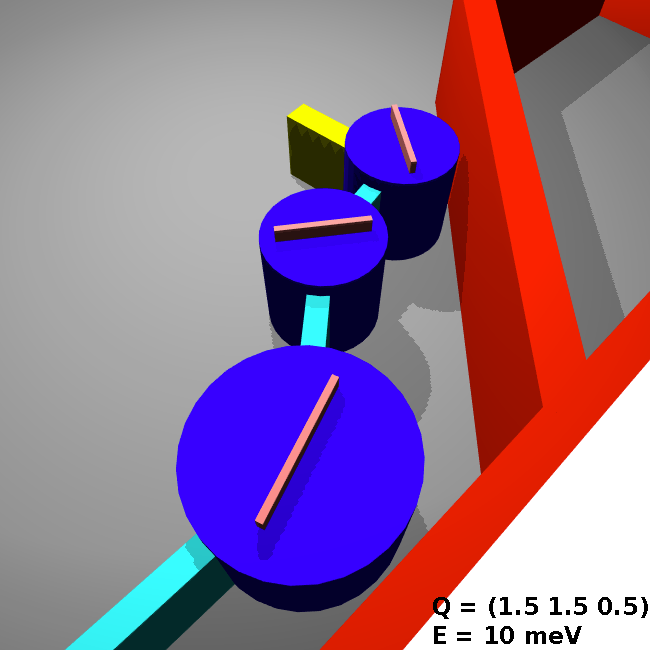
\includegraphics[width = 0.4 \textwidth]{figures/casestudy_15_15_05_10meV}
			\hspace{0.5cm}
			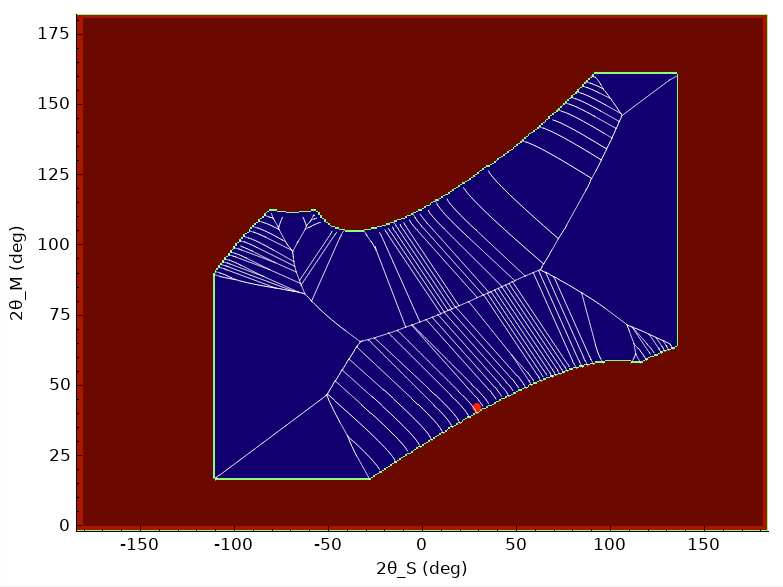
\includegraphics[width = 0.55 \textwidth]{figures/casestudy_15_15_05_10meV_cfg}
		\end{center}
	\caption[Case study: Start position.]{Start position shown in real (left) and in angular configuration space (right), 
		where the red dot indicates the current instrument position. 
		After some measurement the instrument was at a position
		corresponding to the crystal coordinates $Q_\mathrm{start}\,=\,\left(1.5,\ 1.5,\ 0.5\right)\, \mathrm{rlu}$ and 
		energy transfer $E_\mathrm{start}\,=\,10\, \mathrm{meV}$.
		\label{fig:casestudy_start}}
\end{figure}

\begin{figure}[H]
		\begin{center}
			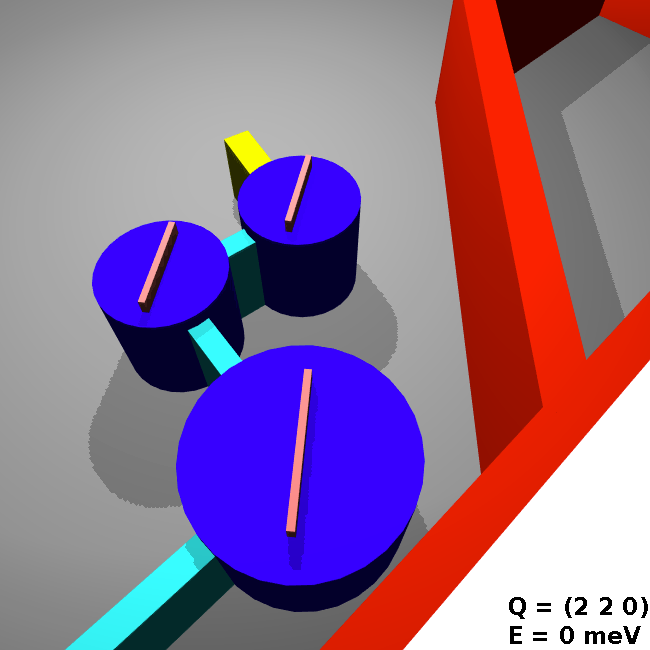
\includegraphics[width = 0.4 \textwidth]{figures/casestudy_2_2_0_0meV}
			\hspace{0.5cm}
			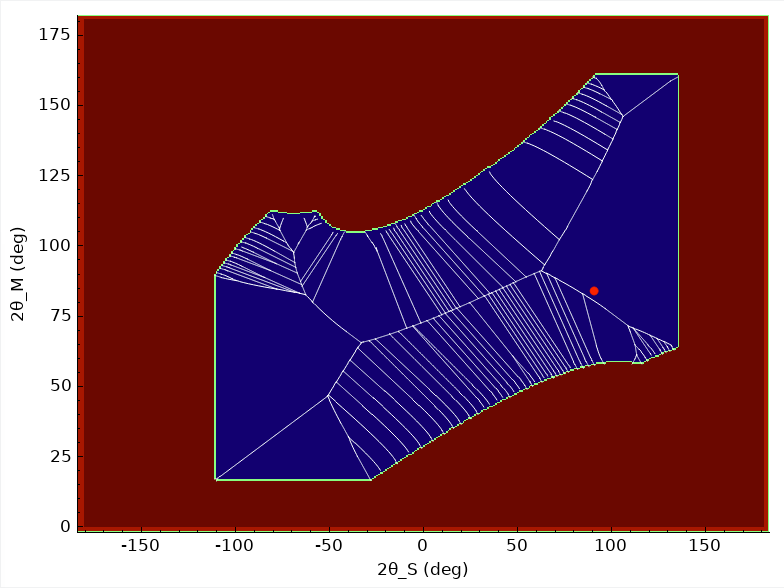
\includegraphics[width = 0.55 \textwidth]{figures/casestudy_2_2_0_0meV_cfg}
		\end{center}
	\caption[Case study: Target position.]{Target position shown in real (left) and in angular configuration space (right). 
		The next set of measurements required the instrument
		to move to the crystal coordinates $Q_\mathrm{target}\,=\,\left(2,\ 2,\ 0\right)\, \mathrm{rlu}$ and 
		energy transfer $E_\mathrm{target}\,=\,0\, \mathrm{meV}$.
		\label{fig:casestudy_target}}
\end{figure}

\begin{figure}[H]
		\begin{center}
			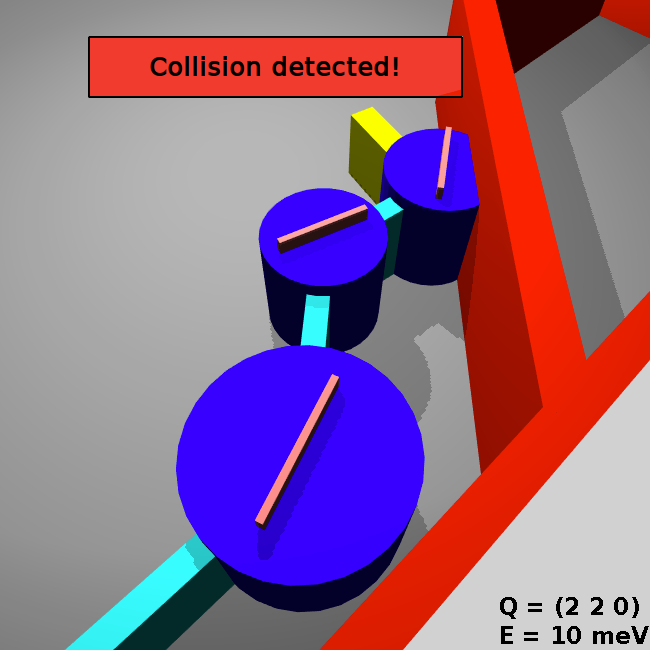
\includegraphics[width = 0.4 \textwidth]{figures/casestudy_2_2_0_10meV}
			\hspace{0.5cm}
			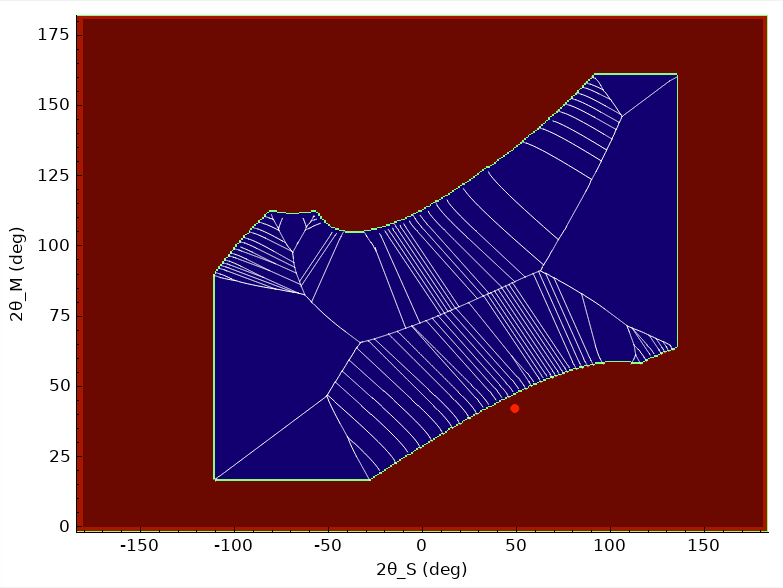
\includegraphics[width = 0.55 \textwidth]{figures/casestudy_2_2_0_10meV_cfg}
		\end{center}
	\caption[Case study: Collision.]{Collision. 
		If one were to drive the instrument directly from $\left(Q_\mathrm{start},\, E_\mathrm{start}\right)$ (Fig. \ref{fig:casestudy_start})
		to $\left(Q_\mathrm{target},\, E_\mathrm{target}\right)$ (Fig. \ref{fig:casestudy_target}), the instrument 
		would collide with the outer wall due to the monochromator motors being much slower than the other 
		motors of the instrument (see text for more explanations).
		\label{fig:casestudy_collision}}
\end{figure}



\paragraph{Solution}
The problem of avoiding the collision with the outer wall  is easily solved by calculating the
path along the skeleton mesh using the software. Figures \ref{fig:casestudy_sequence1} and 
\ref{fig:casestudy_sequence2} show key frames of the driving sequence from the start to the 
target position.
As can be seen in the figure panels, the algorithm ensures that first the monochromator 
(related to the energy) is driven primarily, while the sample scattering angle (related to the momentum) 
is initially driven away from the wall and in the opposite direction than that of its final position (Steps 1-3
in the panels of Fig. \ref{fig:casestudy_sequence1}).
The second part of the sequence primarily drives the sample scattering angle to nearly its
envisaged end position while also still continuing to drive the monochromator (Steps 3-4
in Figures \ref{fig:casestudy_sequence1} and \ref{fig:casestudy_sequence2}).
The third and final part continued driving the sample scattering angle, but drives the monochromator
back a bit, until both reach their target position (Steps 4-5 in Fig. \ref{fig:casestudy_sequence2}).

\begin{figure}[htb]
		\begin{center}
			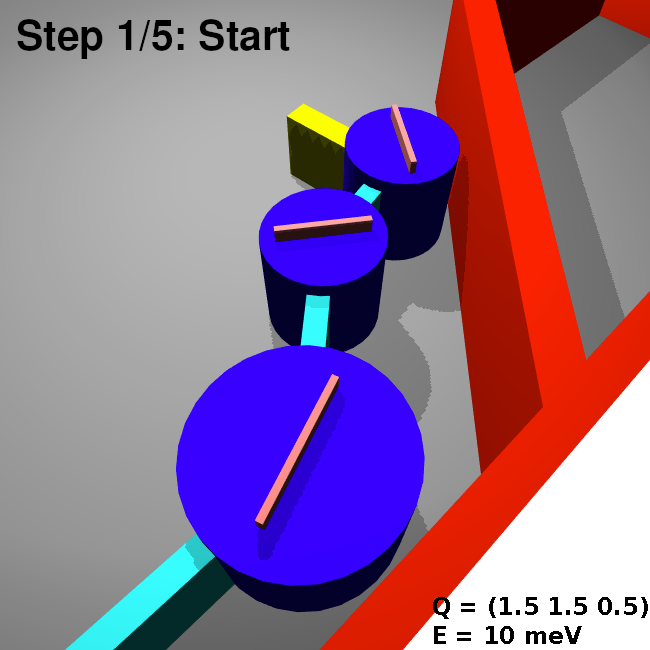
\includegraphics[width = 0.4 \textwidth]{figures/casestudy_step0}
			\hspace{0.5cm}
			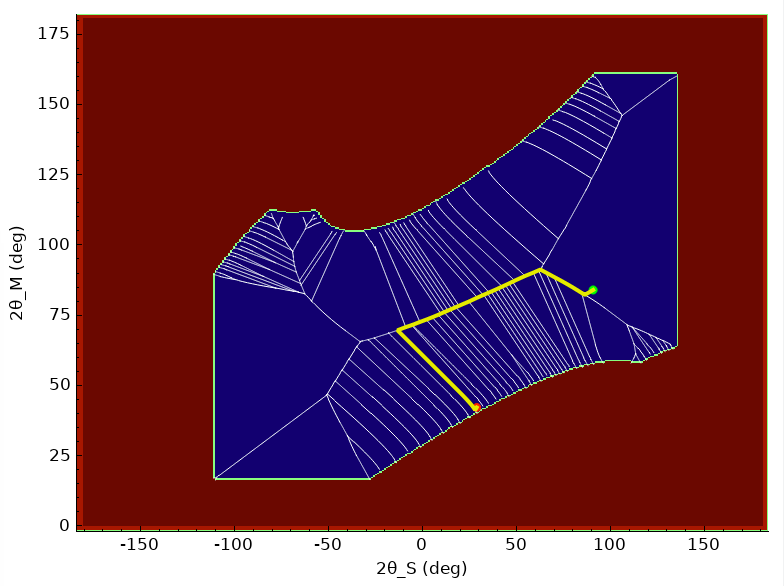
\includegraphics[width = 0.55 \textwidth]{figures/casestudy_path}
			\vspace{0.2cm}
			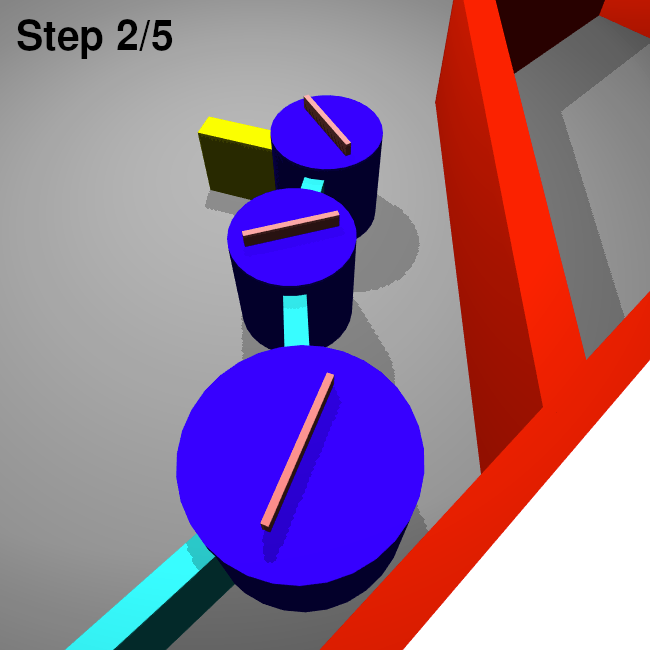
\includegraphics[width = 0.4 \textwidth]{figures/casestudy_step1}
			\hspace{0.5cm}
			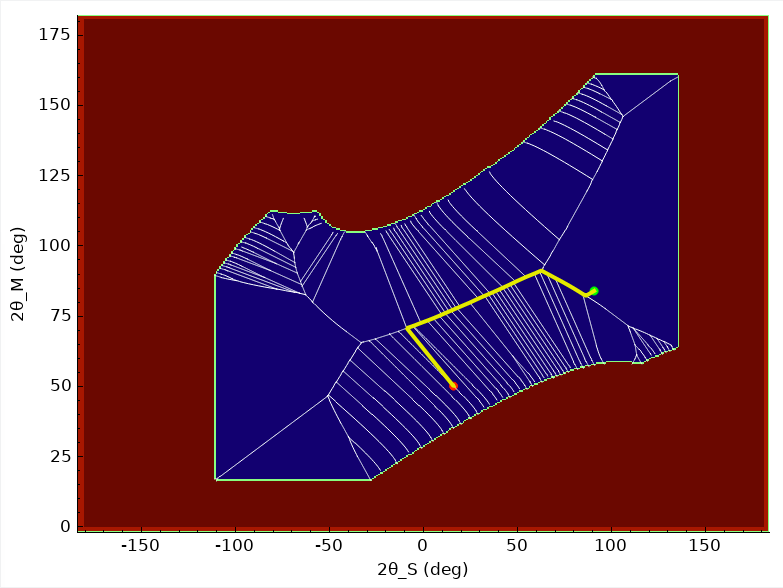
\includegraphics[width = 0.55 \textwidth]{figures/casestudy_step1_cfg}
			\vspace{0.2cm}
			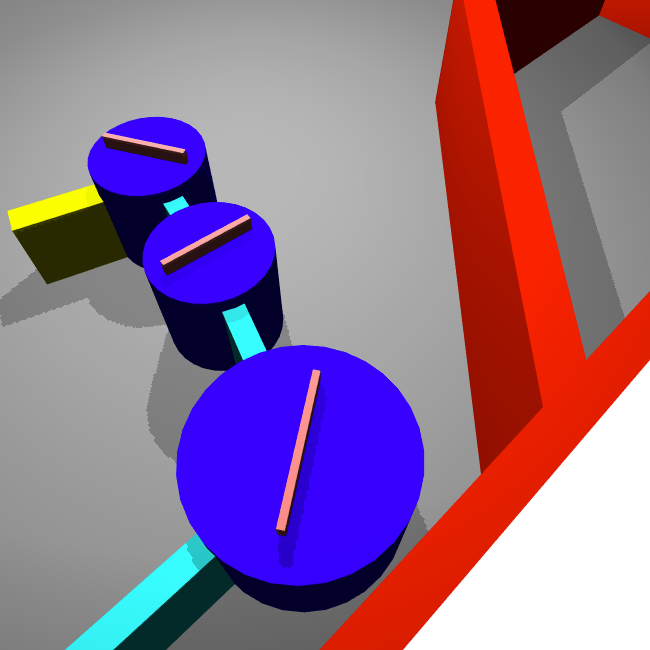
\includegraphics[width = 0.4 \textwidth]{figures/casestudy_step2}
			\hspace{0.5cm}
			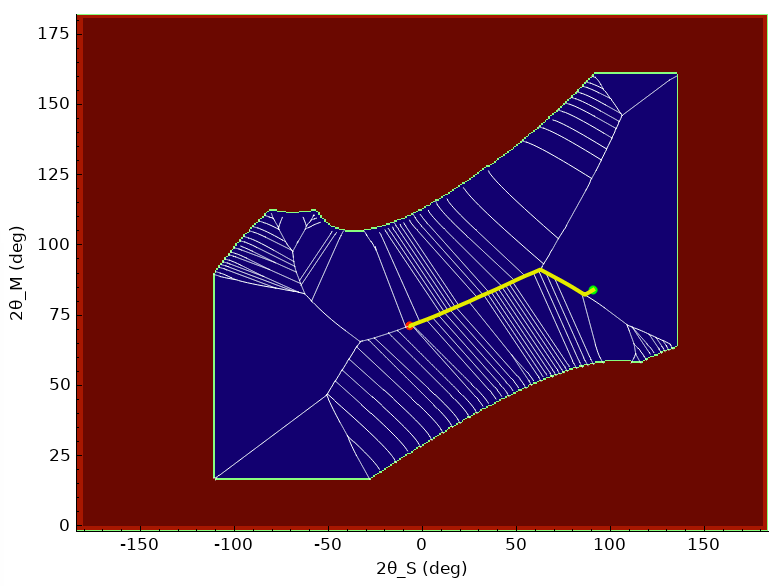
\includegraphics[width = 0.55 \textwidth]{figures/casestudy_step2_cfg}
		\end{center}
	\caption[Case study: Path 1/2.]{The first three steps of the path leading from the start
		to the target position and avoiding the collision with the outer wall. As before, the
		left-hand sides show the real-space instrumental configuration, while the right-hand
		sides show the corresponding angular configuration space with the red dot indicating the
		current instrument position, and the green dot being the target position.
		The calculated optimal path is drawn as a yellow line.
		\label{fig:casestudy_sequence1}}
\end{figure}

\begin{figure}[htb]
		\begin{center}
			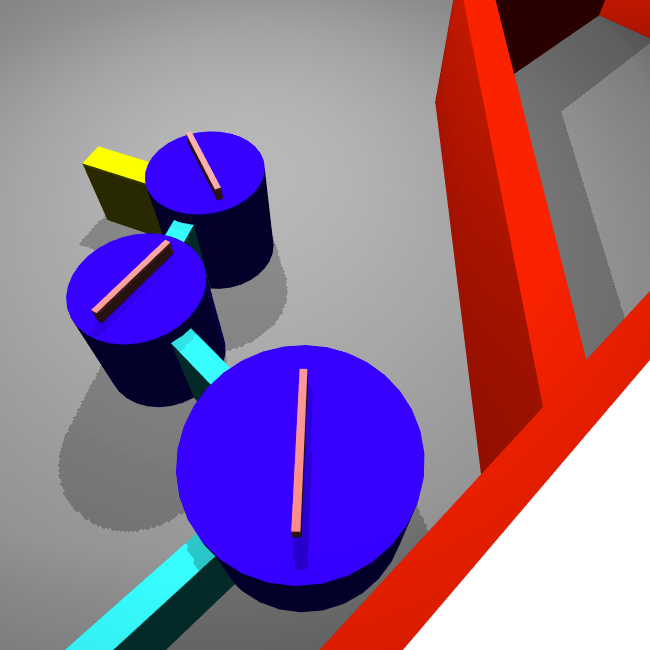
\includegraphics[width = 0.4 \textwidth]{figures/casestudy_step3}
			\hspace{0.5cm}
			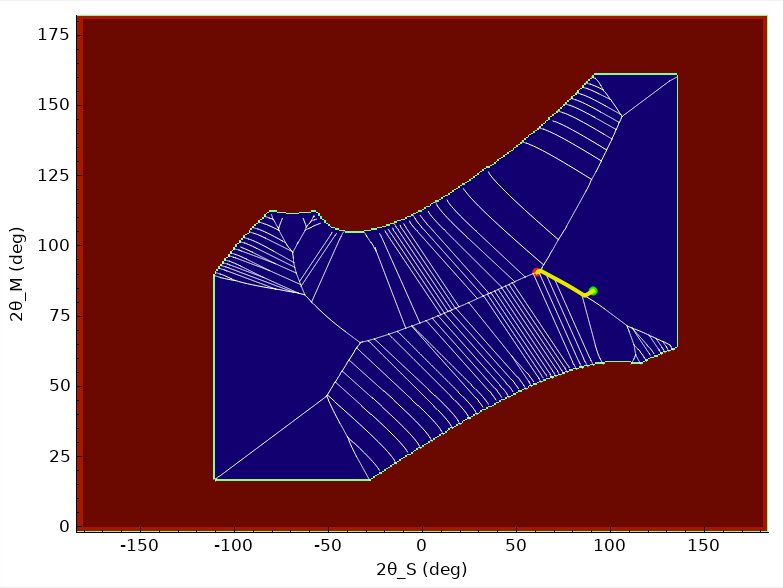
\includegraphics[width = 0.55 \textwidth]{figures/casestudy_step3_cfg}
			\vspace{0.2cm}
			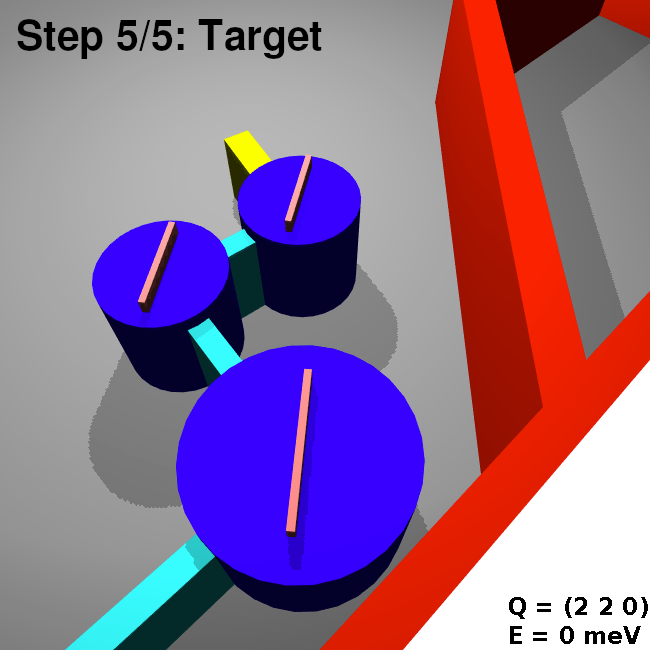
\includegraphics[width = 0.4 \textwidth]{figures/casestudy_step4}
			\hspace{0.5cm}
			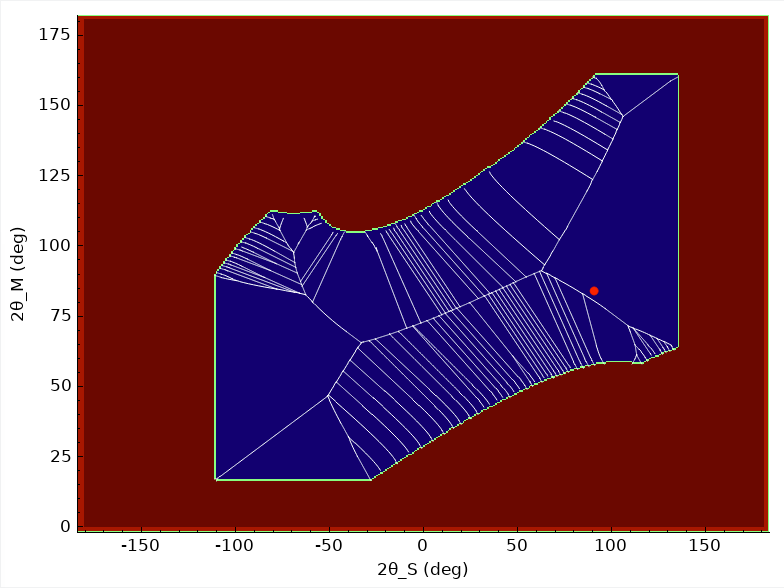
\includegraphics[width = 0.55 \textwidth]{figures/casestudy_2_2_0_0meV_cfg}
		\end{center}
	\caption[Case study: Path 2/2.]{The second two steps of the path leading from the start
		to the target position and avoiding the collision with the outer wall.
		The left-hand sides show the real-space instrumental configuration, while the right-hand
		sides show the corresponding angular configuration space with the red dot indicating the
		current instrument position, and the green dot being the target position.
		The calculated optimal path is drawn as a yellow line.
		\label{fig:casestudy_sequence2}}
\end{figure}



\section{Python scripting interface}
\label{sec:scripting}

In order to allow for a simple way to automatise recurring calculations and workflows, as well as to provide
a possibility for inclusion of the core module (see section \ref{sec:library}) of the present 
software in other tools, a scripting interface has been developed using the interface generator \textit{SWIG} \cite{web_swig}. 
\textit{SWIG} is a tool which parses C or C++ header files and creates a native interface 
for several possible scripting languages, of which we opted for \textit{Python} \cite{Rossum2011, web_python} 
as it has become one of the most popular programming language in neutron science over the last decade.
As the core module already has the structure of a library, the effort to offer scripting functionality
was minimal. Only a few helper functions had to be included in several classes, because \textit{SWIG}
is not yet fully C++20 compliant and had some problems with new language features such as 
template concepts \cite{cppwiki_concepts}.
The \textit{SWIG} interface definition, which maps the C++ classes to corresponding \textit{Python} 
classes of the same name, can be found in the file \lstinline|./scripting/taspaths.i| of the source repository.

\paragraph{Typical workflow}
An example of the full workflow consisting of loading an instrument definition file, creating a path 
mesh and finding the path from a start position in crystal coordinates to a target position is given in listings 
\ref{lst:pyworkflow1}, \ref{lst:pyworkflow2} and \ref{lst:pyworkflow3}.
The native core module is imported into \textit{Python} as the name \lstinline[language=C++]|tas| on line 9 of the script,
instances of its classes are generated for the individual functionalities.
Specifically, the instrument space class from chapter \ref{sec:tasmodel}, which is the representation of the instrument 
and which is furthermore responsible for the local instrument axis coordinate systems, collision detection, as well as 
loading and saving of instrument configurations, is created on line 37. 
Next, the triple-axis and single-crystal calculator class from chapter \ref{ch:xtal} is created on line 51 and is 
used to set-up the instrument scattering senses and a single-crystal coordinate system.
Finally, the path builder class, which has been described in chapter \ref{sec:buildpath}, is created on line 64 
and used in the rest of the script to calculate the path mesh as well as the concrete path between the 
given crystal coordinate points.
The results of the script are shown in Fig. \ref{fig:pyworkflow}, where we employ \textit{Matplotlib} 
\cite{Hunter2007, web_matplotlib} to plot the calculated path and the obstacles in configuration space.

\begin{figure}[htb]
		\begin{center}
			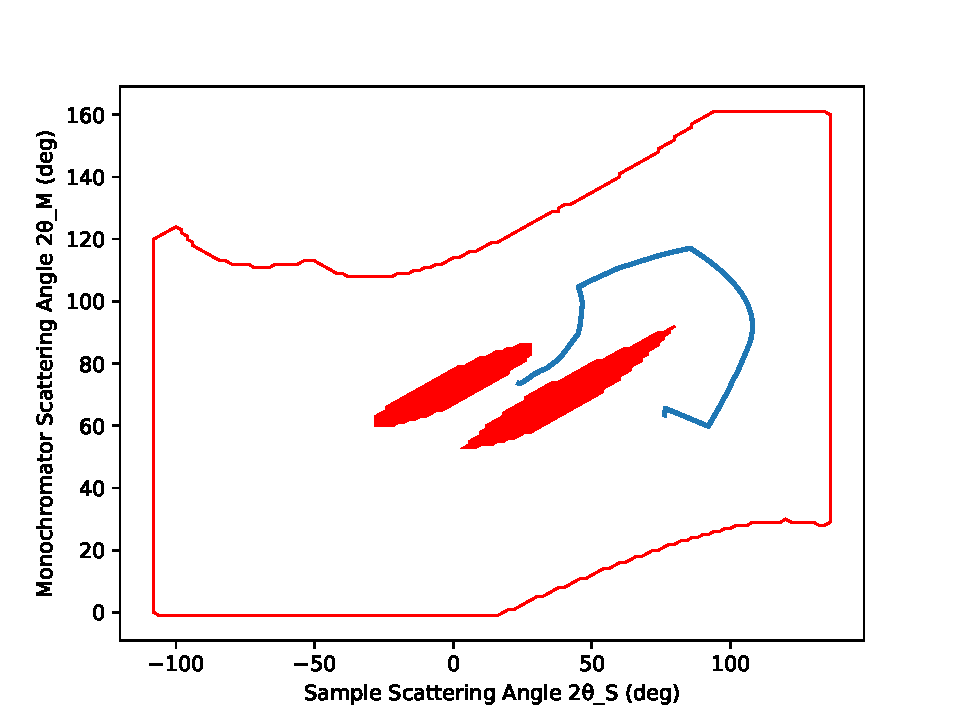
\includegraphics[width = 0.66 \textwidth]{figures/pyworkflow}
		\end{center}
	\caption[Python workflow results.]{Results from the \textit{Python} workflow example of listings
		\ref{lst:pyworkflow1}, \ref{lst:pyworkflow2} and \ref{lst:pyworkflow3}, directly plotted 
		in \textit{Python} using \textit{Matplotlib} \cite{Hunter2007, web_matplotlib}.
		The obstacles are shown as red regions, the calculated instrument path is shown as a blue curve.
		\label{fig:pyworkflow}}
\end{figure}


\begin{listing}[htb]
	\begin{lstlisting} [language = Python, 
		basicstyle = {\scriptsize},
		breaklines = true, tabsize = 4,
		numbers = left, firstnumber = 1, numberstyle={\scriptsize}]
import sys
import os
import math as m

cwd = os.getcwd()
sys.path.append(cwd)

# import native C++ core module
import taspaths as tas

# -----------------------------------------------------------------------------
# helper functions
# -----------------------------------------------------------------------------
def error(msg):
	print("Error: %s" % msg)
	exit(-1)

def warning(msg):
	print("Warning: %s" % msg)
# -----------------------------------------------------------------------------

# -----------------------------------------------------------------------------
# options
# -----------------------------------------------------------------------------
write_pathmesh = False
write_path = False
show_plot = True
file_name = "../res/instrument.taspaths"
# -----------------------------------------------------------------------------

# -----------------------------------------------------------------------------
# load instrument
# -----------------------------------------------------------------------------
print("Loading instrument definition...")

# create the instrument space and load an instrument definition
instrspace = tas.InstrumentSpace()
[file_ok, file_date] = tas.InstrumentSpace.load(file_name, instrspace)

if file_ok:
	print("Loaded \"%s\", dated %s." % (file_name, file_date))
else:
	error("Could not load \"%s\"." % (file_name))

print("Instrument definition loaded.\n")
# -----------------------------------------------------------------------------

# -----------------------------------------------------------------------------
# set-up a sample single-crystal
# -----------------------------------------------------------------------------
tascalc = tas.TasCalculator()
tascalc.SetScatteringSenses(True, False, True)
tascalc.SetSampleLatticeConstants(5, 5, 5)
tascalc.SetSampleLatticeAngles(90, 90, 90, True)
tascalc.UpdateB()
tascalc.UpdateUB()
# -----------------------------------------------------------------------------
	\end{lstlisting}
	\caption[Python workflow example 1/3.]{Script showing an example workflow in \textit{Python}.
	Part 1 of 3: Set-up of the instrument and the sample crystal.
	\label{lst:pyworkflow1}}
\end{listing}



\begin{listing}[htb]
	\begin{lstlisting} [language = Python, 
		basicstyle = {\scriptsize},
		breaklines = true, tabsize = 4,
		numbers = left, firstnumber = 58, numberstyle={\scriptsize}]
# -----------------------------------------------------------------------------
# build path mesh
# -----------------------------------------------------------------------------
print("Building path mesh...")

# create the paths builder object
builder = tas.PathsBuilder()
builder.AddConsoleProgressHandler()
builder.SetInstrumentSpace(instrspace)
builder.SetTasCalculator(tascalc)
print("Path builder uses %d threads." % builder.GetMaxNumThreads())

# angular ranges to probe
angle_padding = 4.
a2_delta = 1./180.*m.pi
a4_delta = 2./180.*m.pi
a2_begin = 0. - angle_padding*a2_delta
a2_end = m.pi + angle_padding*a2_delta
a4_begin = -m.pi - angle_padding*a4_delta
a4_end = m.pi + angle_padding*a4_delta

if not builder.CalculateConfigSpace(
	a2_delta, a4_delta,
	a2_begin, a2_end,
	a4_begin, a4_end):
	error("Angular configuration space could not be calculated.")

if not builder.CalculateWallContours(True, False):
	error("Obstacle contours could not be calculated.")

if not builder.CalculateLineSegments():
	error("Line segments could not be calculated.")

if not builder.CalculateVoronoi(False):
	error("Voronoi diagram could not be calculated.")

print("Finished building path mesh.\n")
# -----------------------------------------------------------------------------

# -----------------------------------------------------------------------------
# set-up the start and target coordinates of a path
# -----------------------------------------------------------------------------
print("Calculating path...")

tascalc.SetKf(1.4)
start_angles = tascalc.GetAngles(0.5, 0., 0., 1.)
target_angles = tascalc.GetAngles(1.5, -0.5, 0., 2.5)

# take absolute angles
start_angles.monoXtalAngle = abs(start_angles.monoXtalAngle)
start_angles.sampleXtalAngle = abs(start_angles.sampleXtalAngle)
start_angles.sampleScatteringAngle = abs(start_angles.sampleScatteringAngle)
target_angles.monoXtalAngle = abs(target_angles.monoXtalAngle)
target_angles.sampleXtalAngle = abs(target_angles.sampleXtalAngle)
target_angles.sampleScatteringAngle = abs(target_angles.sampleScatteringAngle)

print("Start angles: a1 = %.2f deg, a5 = %.2f deg, a3 = %.2f deg, a4 = %.2f deg." % (
	start_angles.monoXtalAngle / m.pi*180.,
	start_angles.anaXtalAngle / m.pi*180.,
	start_angles.sampleXtalAngle / m.pi*180.,
	start_angles.sampleScatteringAngle / m.pi*180.))

print("Target angles: a1 = %.2f deg, a5 = %.2f deg, a3 = %.2f deg, a4 = %.2f deg." % (
	target_angles.monoXtalAngle / m.pi*180.,
	target_angles.anaXtalAngle / m.pi*180.,
	target_angles.sampleXtalAngle / m.pi*180.,
	target_angles.sampleScatteringAngle / m.pi*180.))
# -----------------------------------------------------------------------------
	\end{lstlisting}
	\caption[Python workflow example 2/3.]{Script showing an example workflow in \textit{Python}.
	Part 2 of 3: Calculation of the path mesh and the start and target positions from their crystal coordinates.
	\label{lst:pyworkflow2}}
\end{listing}


\begin{listing}[htb]
	\begin{lstlisting} [language = Python, 
		basicstyle = {\scriptsize},
		breaklines = true, tabsize = 4,
		numbers = left, firstnumber = 126, numberstyle={\scriptsize}]
# -----------------------------------------------------------------------------
# find path
# -----------------------------------------------------------------------------
path = builder.FindPath(
		start_angles.monoXtalAngle * 2., start_angles.sampleScatteringAngle,
		target_angles.monoXtalAngle * 2., target_angles.sampleScatteringAngle)
if not path.ok:
	error("No path could be found.")

builder.SetSubdivisionLength(0.5)
vertices = builder.GetPathVerticesAsPairs(path, True, True)

print("Finished calculating path.\n")
# -----------------------------------------------------------------------------

# -----------------------------------------------------------------------------
# output and plotting
# -----------------------------------------------------------------------------
# write the path mesh vertices to a file
if write_pathmesh:
	if not builder.SaveToLinesTool("lines.xml"):
		warning("Could not save line segment diagram.")

# write the path vertices to a file
if write_path:
	with open("path.dat", "w") as datafile:
		for vertex in vertices:
			datafile.write("%.4f %.4f\n" % (vertex[0], vertex[1]))

# plot the angular configuration space
if show_plot:
	import matplotlib.pyplot as plt

	# plot obstacles
	numgroups = builder.GetNumberOfLineSegmentRegions()
	print("Number of regions: %d." % numgroups)
	for regionidx in range(numgroups):
		region = builder.GetLineSegmentRegionAsArray(regionidx)
		x1, y1, x2, y2 = zip(*region)
		plt.fill(x1, y1, "-", linewidth = 1,
			fill = not builder.IsRegionInverted(regionidx), 
			color = "#ff0000")

	# plot path
	x, y = zip(*vertices)
	plt.xlabel("Sample Scattering Angle 2\u03b8_S (deg)")
	plt.ylabel("Monochromator Scattering Angle 2\u03b8_M (deg)")
	plt.plot(x, y, "-", linewidth=2)

	plt.show()
# -----------------------------------------------------------------------------

	\end{lstlisting}
	\caption[Python workflow example 3/3.]{Script showing an example workflow in \textit{Python}.
	Part 3 of 3: Calculation of the path between the start end target positions and plotting.
	\label{lst:pyworkflow3}}
\end{listing}


\section{Summary}
The modular design of the software keeps the interface code separate from the calculation core.
Several different types of interfaces were discussed in this chapter, most prominently the graphical 
user interface, which provides the most accessible way for the end user to interact with the software.
We demonstrated a typical situation of the instrument colliding with an outer wall, which arose 
during one of our past measurements, and which can be solved graphically using the software's GUI.
A separate scripting interface makes it easy to automatise calculations on the command line and 
to interface with other software tools.

Having outlined the entirety of the software, what remains to be done in the next chapter
is a description of the tools used to ensure that it stays bug-free, for example when
introducing new features to the core module.
